\documentclass[11pt,a4paper]{report}
\usepackage{titlesec}
\usepackage{listings}
\usepackage{graphicx}
\usepackage{wrapfig}
\usepackage[hidelinks]{hyperref}
\usepackage{tikz}
\usetikzlibrary{calc}
\usepackage[utf8]{inputenc}
\usepackage[left=3cm,right=3cm]{geometry}
\usepackage{calc}
\usepackage{eso-pic}
\usepackage{placeins}
\usepackage[document]{ragged2e}
\usepackage{titling}
\usepackage{float}

\begin{document}
    
\renewcommand\bibname{References}

\titleformat{\chapter}{\bfseries\huge\centering}{}{0pt}{}{\huge}
\titlespacing*{\chapter}{0pt}{-60pt}{40pt}
\setlength{\parindent}{2em}
\setlength{\parskip}{1em}

\newenvironment{myindentpar}[1]%
  {\begin{list}{}%
          {\setlength{\leftmargin}{#1}}%
          \item[]%
  }
  {\end{list}}

\title{Android Application Implementing ListView Using Linked List}

\author{Kashish Srivastava (185014)\\
        \and 
        Dipesh Kumar (185015)\\
        \and
        Akash Rana (185034)
}

\date{July 2020}



\pagestyle{plain}

\begin{titlepage}
    \begin{center}

        \Huge{\textbf{Android Application Implementing ListView Using Linked List}}
 
        \vspace{0.5cm}
        
        \normalsize
       
        \vspace{10pt}
        
    	Data Structures\\
        CSD-223

        
        
        \vspace{15pt}
        
\includegraphics[height=5cm]{./img/logo.png}
        
        \vspace{10pt}
        \textit{Submitted by:}

            Kashish Srivastava (185014)\\
            Dipesh Kumar (185015)\\
            Akash Rana (185034)
        \vspace{5pt}
        
        CSE (4 Year) : 
        4\textsuperscript{th} Semester
 
        \vspace{15pt}
 
        Under the guidance of
        
        \vspace{5pt}
        
        \textbf{Dr. Nitin Gupta }\\
        Assistant Professor, CSE Department\\
        National Institute of Technology, Hamirpur\\
 
        \vspace{25pt}
        
        \large
 
        Department of Computer Science and  Engineering\\
        National Institute of Technology, Hamirpur\\
      
    \end{center}
\end{titlepage}

\chapter{Abstract}		

Our goal was to develop a android application using list and file structure implementation as per instructions. This Android application is basically coded in Kotlin. This Android application will provide our 
student and other people with the brief information of each and every department (i.e about different branches of engineering that are available in our institute) to have the better idea of every department of 
our institute and its courses available in that respective department. By developing this Android application, our basic idea was to provide the clear idea of how linked list, queue, stack and sets can be used 
to develop a well working an application.
\vspace{5pt} 


\tableofcontents

\chapter{Introduction}

The era of mobile technology opens the window to the android app development. The websites are vanishing and the mobile phones are emerging. It`s high time to changeform conventional form websites to apps, which 
has become the part of our daily routine. We are here introducing self made android application which would be a miniature part of our college website. It not only works as a website but also as a small college 
management software. This android application will provide our student and other managing staffs with the proper information of each and every department and of about its courses and placement. This android 
application is also a mobile version of the part of our institute official website.

This android application also uses different data structures in the development of the same. The data structures used in its development are linked list, queue, arrays, hash table etc. These all the data structure
 are pre provided by the android development for the development of such application.
 
 List view is used in this application to groups several items and display them in vertical scrollable list which is a list of department of our institute and similarly linked list is used in this application to 
 link last element with the recent one and also it allocates memory dynamically and hence these data structures are used in our application.

This project is basically designed to provide the better idea of how data structures i.e linked list,list view,hash table and arrays can be used to develop real life android application for the betterment of 
the coming youth.
\vskip 30cm



\chapter{Requirements and Installation}
	
The software and programming languages that are required to build an android application and we should also have prior knowledge about the following:-

\subsection*{\Large{Kotlin 1.32}}

Kotlin is a statically typed programming language for Java Virtual Machine (JVM) and JavaScript. Described as a general-purpose language, Kotlin introduces functional features to support Java
 interoperability. The Kotlin project was born out of the aspiration for heightened productivity. The goal was to improve the coding experience in a way that was both practical and effective.

\subsection*{\Large{Android Studio 3.6.1}}

Android Studio is an IDE, which is essentially an interface where you can enter your code (primarily Java or Kotlin) and access all the different tools necessary for development. 
Android Studio allows you to access libraries and APIs from the Android software development kit(SDK`s).

\subsection*{\Large{Android Virtual Device}}

An Android Virtual Device (AVD) is a configuration that defines the characteristics of an Android phone, tablet, Wear OS, Android TV, or Automotive OS device that you want to simulate in
 the Android Emulator. The AVD Manager is an interface you can launch from Android Studio that helps you create and manage AVDs.



 \chapter{Workflow and Components used}

The basic workflow to develop a working android application can be explained using the image given below:-
\begin{figure}[H]
	\centering
	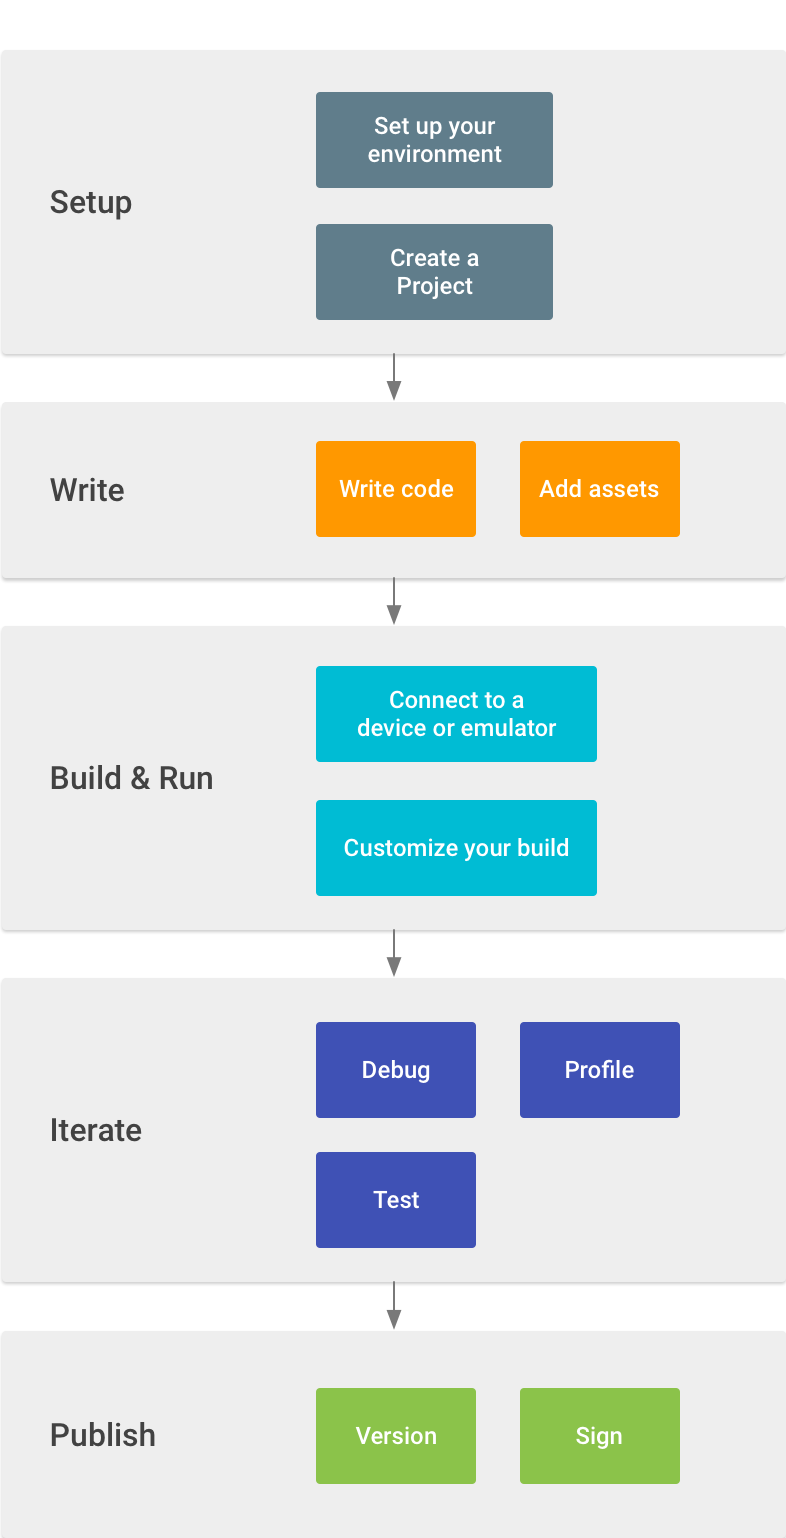
\includegraphics[scale=0.3]{./img/developer-workflow_2x.png}
	\caption{The workflow to develop an application .}
\end{figure}
\vskip 7cm



\textbf{{\large{Components used for Building the android application}}}
\section{ListView (View)}
\vskip 0.5cm
Android ListView is a view which contains the group of items and displays in a scrollable list. ListView is implemented by importing android.widget.ListView class. 
ListView is a default scrollable which does not use other scroll view.

ListView uses Adapter classes which add the content from data source (such as string array, array, database etc) to ListView. Adapter
 bridges data between an AdapterViews and other Views (ListView, ScrollView etc).

\begin{figure}[H]
	\centering
	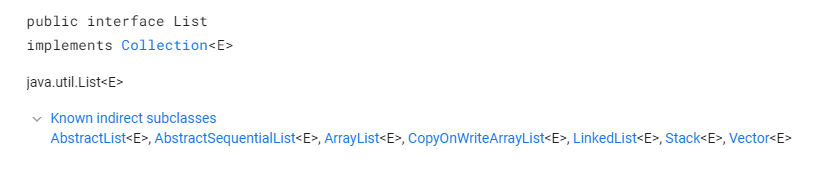
\includegraphics[scale=0.75]{./img/Screenshot (146).png}
\end{figure}


\section{Linked List (Data Structure)}
Doubly-linked list implementation of the List and Deque interfaces. Implements all optional list operations, and permits all elements (including null).

All of the operations perform as could be expected for a doubly-linked list. Operations that index into the list will traverse the list from the beginning or the end, whichever is closer to the specified index.
	\begin{figure}[H]
		\centering
		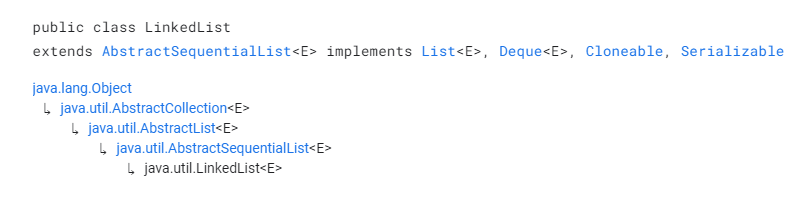
\includegraphics[scale=0.75]{./img/Screenshot (145).png}
	\end{figure}


\chapter{Conclusion}
This Project was a great opportunity for us to discover new fields and ways of working.Doing this project was very interesting since our skills were really complementary. Learning kotlin and languages for this project was truly enthralling and opened new vistas for us. Indeed, it forced us to understand sound synthesis from scratch, something that always interested us. We started the project with no clear objective, and our main goal at the beginning was to build an application which will further benefit our youth in the coming future
\begin{figure}[H]
  \centering
  \begin{minipage}[b]{0.4\textwidth}
    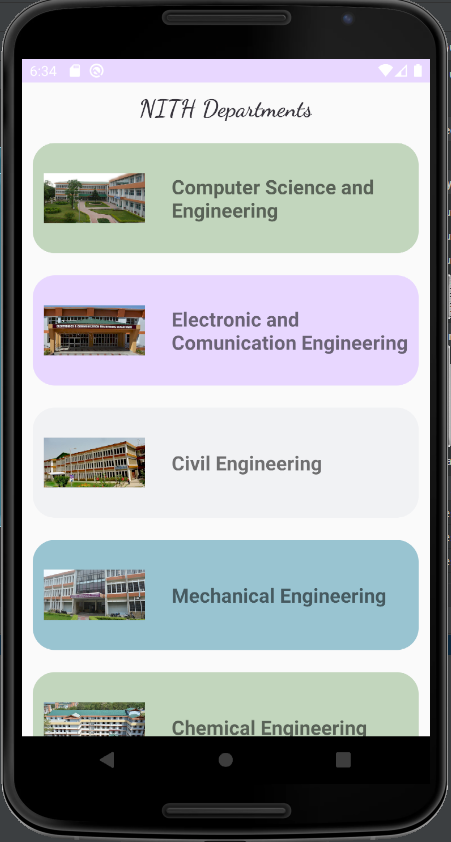
\includegraphics[width=\textwidth]{./img/Capture1.png}
    \caption{user interface 01}
  \end{minipage}
  \hfill
  \begin{minipage}[b]{0.4\textwidth}
    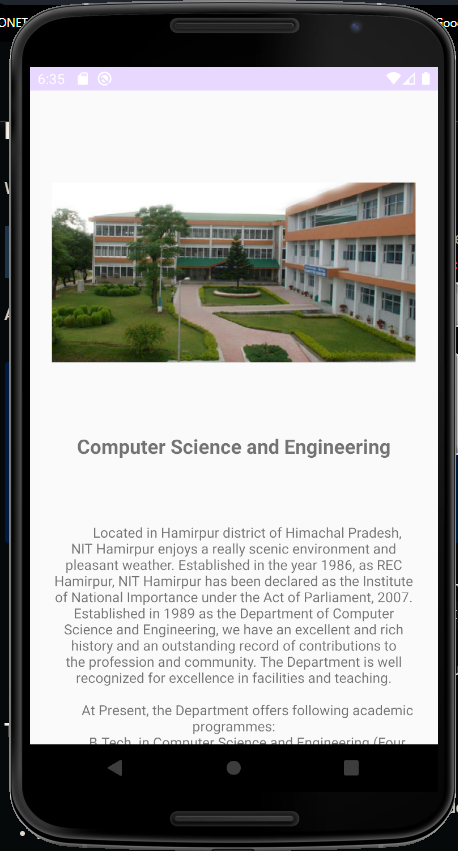
\includegraphics[width=\textwidth]{./img/Capture2.png}
    \caption{user interface 02}
  \end{minipage}
\end{figure}



\chapter{References}
\vskip 1cm
{\large{The source code and other files related to this project can  be found at}\\
\url{https://github.com/cannibalcheeseburger/ds-app.git}\\
\vskip 1cm
\large{We used following references while working with this project:-}
\begin{itemize}
	\item  Natarajan Raman, Eunice Adutwumwaa Obugyei, Learning Kotlin by Building Android Applications: Explore the Fundamentals of Kotlin by Building Real-world Android Applications.
	\item Samuel Urbanowicz: Kotlin Standard Library Cookbook.
	\item \url{https://youtu.be/PJ3RdfJ4Np8}
	\item \url{http://developer.android.com/reference/packages.html}
	\item \url{http://developer.android.com/guide/topics/ui/index.html}
\end{itemize}
}

\end{document}